\chapter{Risk Management}\label{ch:Risk Management}

Når det gælder software projekter, eller i det hele taget projekter generelt, er der flere risici, som bør identificeret, overvejet og analyseret. Risici er mulige negative afvigelser fra planen.\cite{SlideRiskAnalysis} I dette afsnit, vil gruppen danne et overblik over forskellige metoder, som kan bruges til at identificere risici, samt hvordan risici er blevet analyseret ift. projektet.

\section{Risici}

Der er mange mulige metoder til at analysere hvilke risici et team står overfor. Fælles for dem er, at starte ud med at identificere mulige risici.
Identificering af ricisi kan blive skåret ned i meget mindre steps. \cite{SlideRiskAnalysis} Disse steps fokuser på at stille en række sprøgsmål ind til hvilket slags projekt det er, hvor mange der kommer til at benytte det og hvad der vil ske hvis det ikke virker? Hertil, reflekterer over tidligere projekter, om der var noget der teamet burde tage med? Og til sidst, beskrive det i ‘cause, event and effect’. Identificerings processen er i sig selv, en brainstorming process.

Det næste punkt, efterfulgt af at identificere, er vurderer risici. Vurdering af risici gennemgår 2 punkter: Det ene estimering, og det andet evaluering. Estimering dækker sandsynligheden for risici, hvilken effekt det vil have for både trusler og muligheder. Evaluering er når man samler alle risici og danner en risiko værdi for hele projektet.

%Husk at det centrale i dette kapitel er hvilke risici vi har identificeret - dernæst hvilke metoder, og hvordan risici er håndteret.

\section{Boehm}

Boehm skemaet danner et bedre overblik over det metodevalg, som teamet har taget. Da det ikke altid er den agile metode, der er det bedste valg til et projekt er det vigtigt at identificere hvilke risici, der kan opstå ved netop at benytte den agile tilgang. En fejl teamet kan begå, er eksempelvis at automatisk gå ud fra, at en agil tilgang er det bedste valg. For at finde det bedste valg for dette projekt, har vi benyttet Boehm skemaet, til at finde hvor gruppen ligger på skemaet, og hvilken metode der kan vælges ud fra skemaet.
Teamet er på 4 personer så størrelsen på personel er meget lille, så disse to punkter er tættere på midten af skemaet. Vi er i et meget behageligt projekt, da hvis noget går galt, vil det for det første hverken koste et eller flere liv, men det vil heller ikke påvirke økonomisk status, beboelses status eller fysisk helbred. Kigger vi i det hele taget på Boehm skemaet, bliver det hurtigt tydeligt, at teamet falder ind under de røde linjer og derfor den agile tilgang være fordelagtig.

\begin{figure}
    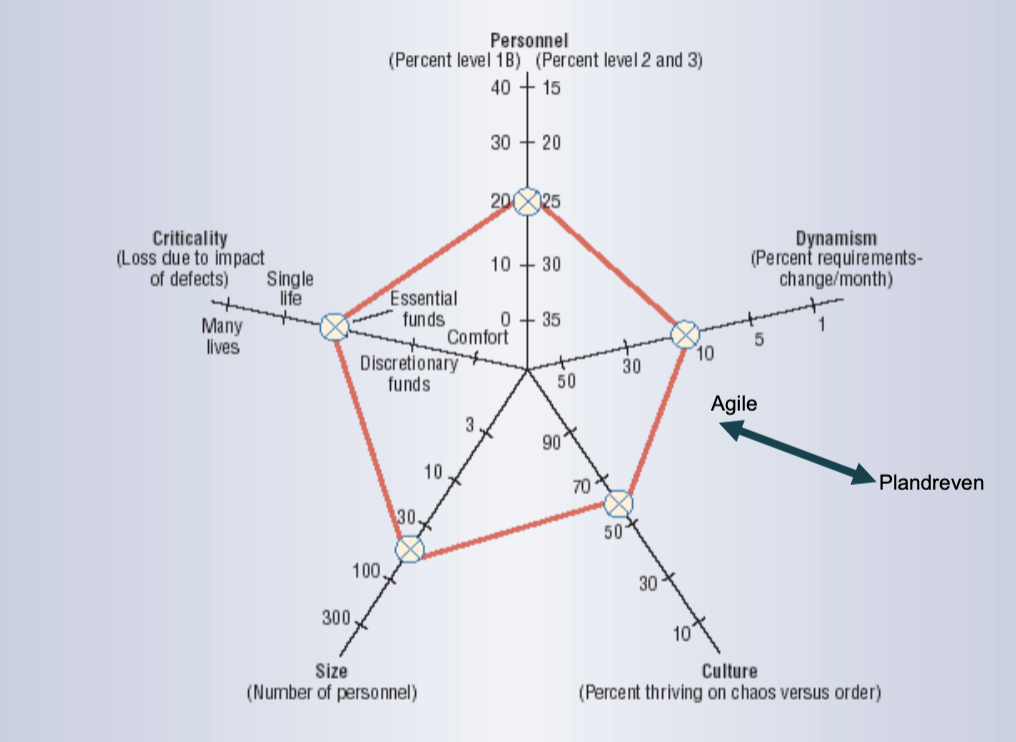
\includegraphics[width=\linewidth]{figures/Boehm.png}
    \caption{Boehm's kritiske faktor.}
    \label{fig:Boehm}
\end{figure}

\begin{figure}
    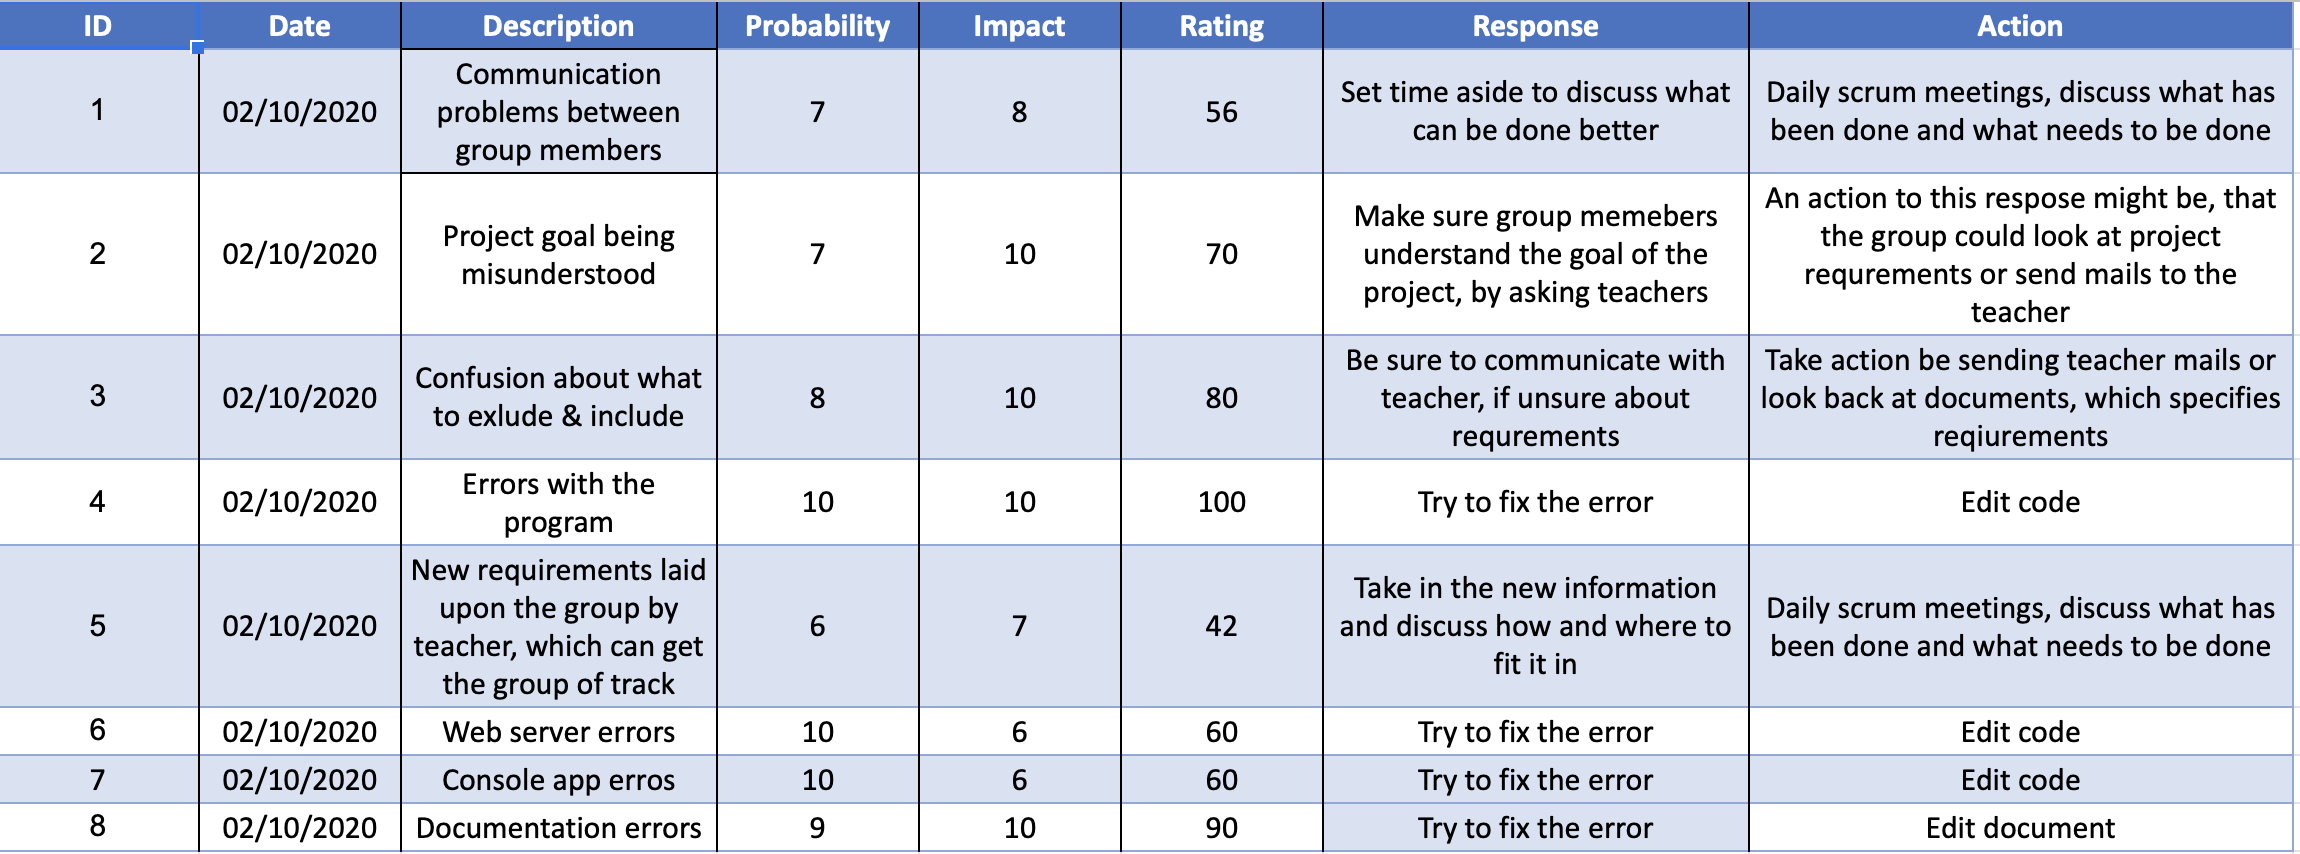
\includegraphics[width=\linewidth]{figures/RiskRegister.png}
    \caption{Teamets Risk Register}
    \label{fig:Risk}
\end{figure}



\section{Identificerede risici}

På figur \ref{fig:Risk} er der dannet et risk register, for dette projekt. For oprettelsen af denne risk register, har teamet, som det første identificerede risici, som beskrevet under ‘Description’. Dette blev gjort ved brug af brainstorming og reflektion, fra tidligere projekter. Efterfuldt, har teamet vurderet risici, ved at gennemtænke hvilken sandsynligheden på en risici og hvilken indvirkning det her på projektet. Når både sandsynligheden og indvirkningen er vurderet, kan vi rankere en risici ved at gange de to. Til sidst har gruppen gennemtænkt det bedste respons, med en kort beskrivelse til en hver risici. Herefter er der beskrevet hvad teamet skal gøre, når den bestemte risici opstår. 

Med dette, er det vigtigt at sørge for projektet ikke bare er sikkert, men også af god kvalitet. Som vi vil kigge nærmere på, når vi har været igemmen hvordan arkitekturen er opsat. 